
\chapter{Rys historyczny}
\label{sec:hisotryMap}

Pomimo że w obecnych czasach codziennie mamy kontakt z mapami i uznajemy je za normalny przedmiot codziennego użytku to nie zawsze tak było. W histori człowieka można znaleść okresy czasu kiedy kartografia była nieznana, a świadomość człowieka o otaczajacym go świecie ograniczała się jedynie do tego co mógł zobaczyć przy pomocy swoich oczu.

Pierwsze malowidła które można uznać za graficzną reprezentację otoczenia archeolodzy napotkali w okolicach Pavloc (Czechy), datowaną są one na 25 wiek przed naszą erą \cite{pre2} . Na 14 wiek p.n.e datowane są wykopaliska w Navarre(Hiszpania) obejmujące rysunki na piaskowcu \cite{pre1}.

Jeszcze w XIV kartografia była bardzo ograniczona, mapy którymi posługiwano się nie były zbyt dokładne. 12 października 1410 gdy Krzysztof Kolumb dotarł do brzegów wyspy San Salvador uznał ją za jedną z wysp japońskich \cite{columb}. Aby lepiej zrozumieć powód tej pomyłki wystarczy spojrzeć na mapę stworzoną w XV wieku przez kartografa Henricusa Martellusa \ref{fig:worldMap1}. Widzimy na niej że m.in. obie ameryki nie były znane uwczesnym ludziom.

\begin{figure}[H]
  \centering
    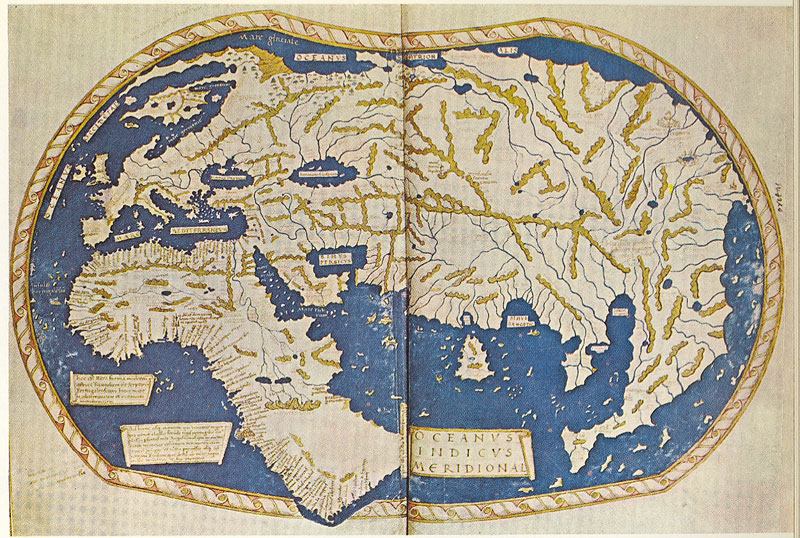
\includegraphics[width=100mm]{ge/worldMap1.jpg}
  \caption{Mapa świata z 1489 roku.}
  \label{fig:worldMap1}
\end{figure}
